\section{Properties of Probability measures}
Let $(\Omega, \mathcal{F}, \mathbb{P})$ be a probability space and $\mathbb{P} : \mathcal{F} \to [0, 1]$.

\begin{definition}[Countable additivity]
    P3 : $\mathbb{P}(\bigcup_{n \in \mathbb{N}} A_n) = \sum_{n \in \mathbb{N}} \mathbb{P}(A_n)$ for $(A_n)_{n \in \mathbb{N}}$ disjoint.
\end{definition} 

\begin{question}
    What if the sets are not disjoint?
\end{question} 

\subsection{Countable sub-additivity}

\begin{proposition}[Countable sub-additivity] \label{prp:subadditivity}
    Let $(A_n)_{n \in \mathbb{N}}$ be a sequence of events in $\mathcal{F}$.
    Then
    \begin{align*}
        \mathbb{P}\left(\bigcup_{n \in \mathbb{N}} A_n\right) \leq \sum_{n \in \mathbb{N}} \mathbb{P}(A_n).
    \end{align*} 
\end{proposition} 

May also be called a \emph{union bound}.

\emph{Intuition}:
\begin{figure}[h] 
    \centering 
    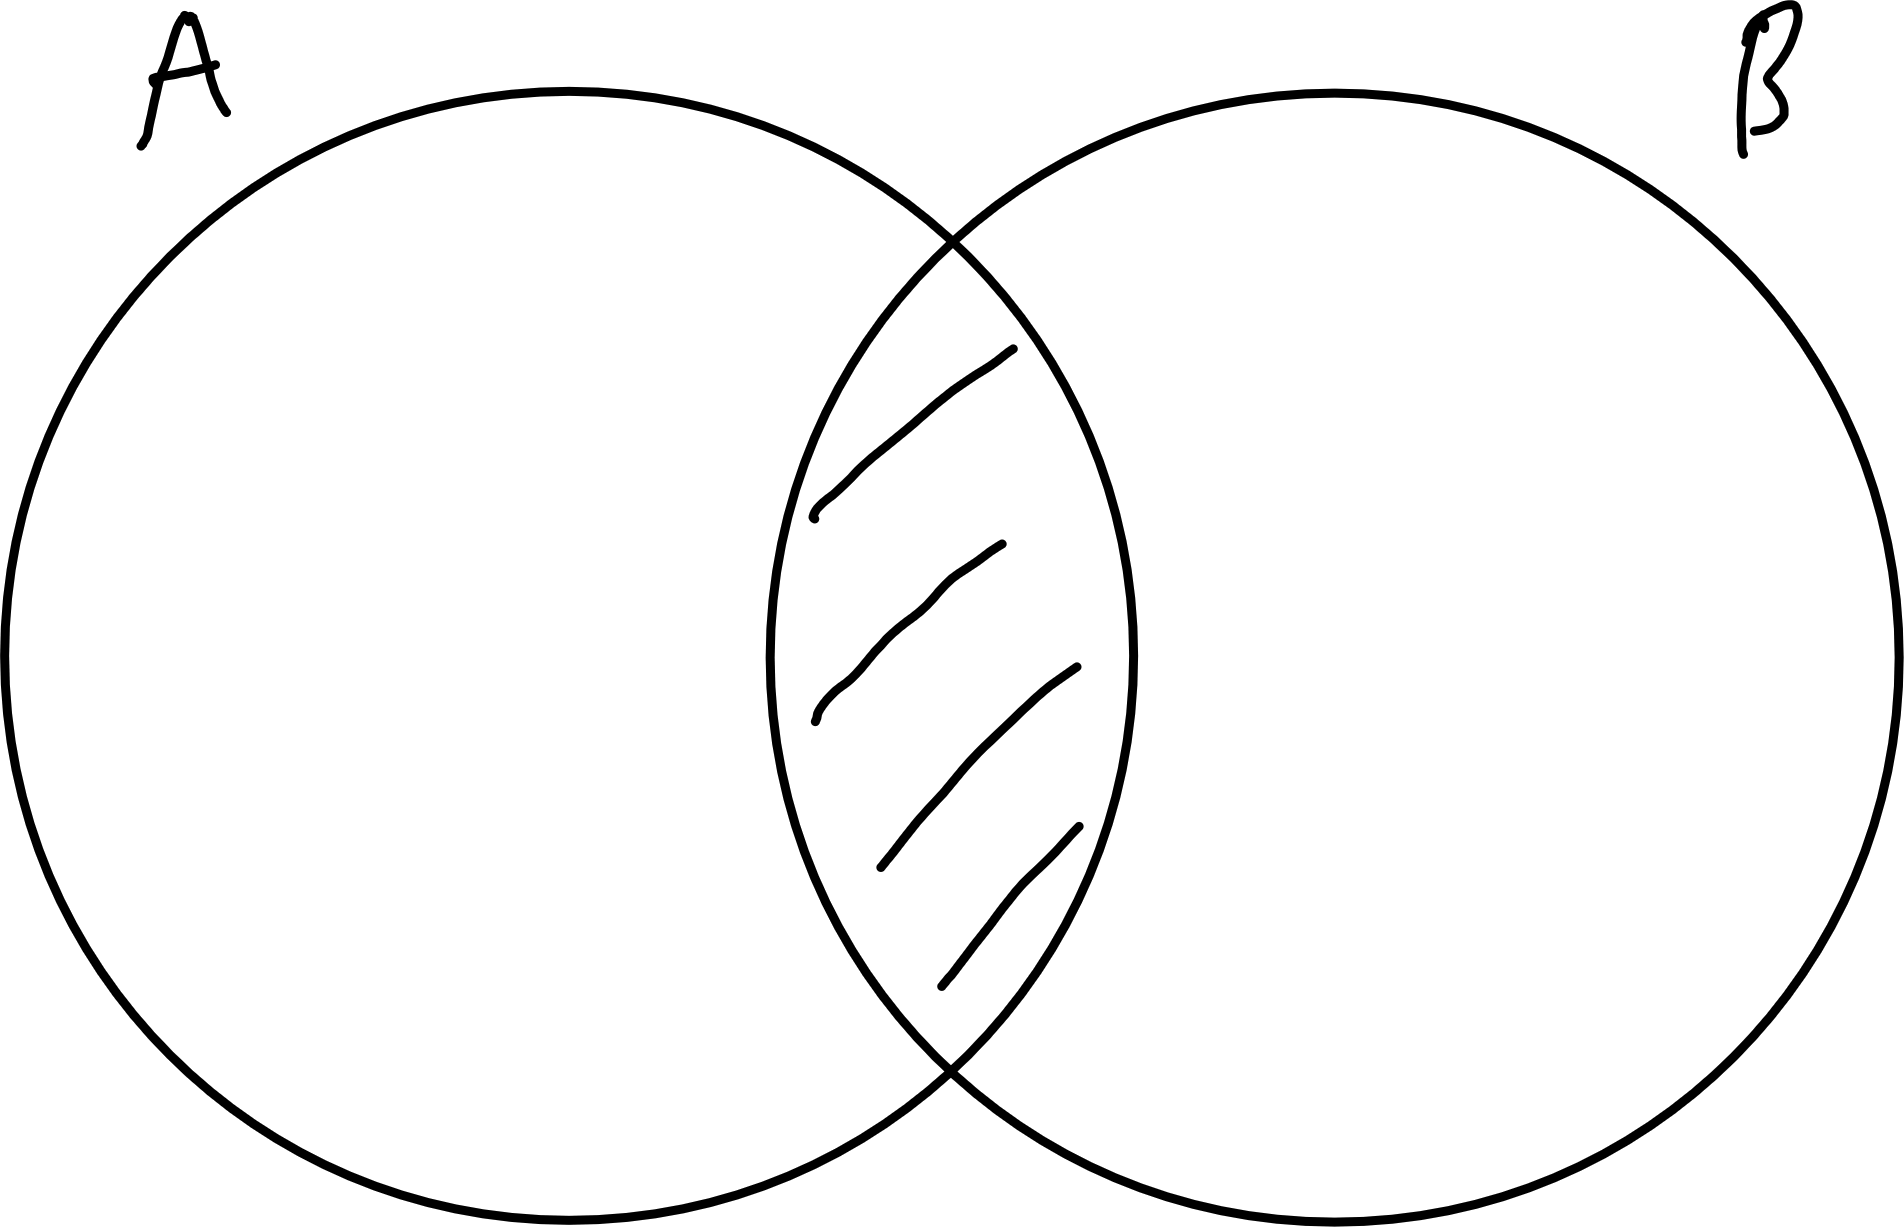
\includegraphics[height=5cm]{03-venn-diagram} 
\end{figure}

$\sum_{n \in \mathbb{N}} \mathbb{P}(A_n)$ ``double counts" some sub-events.

\begin{proof}
    \emph{Idea}: Rewrite $\bigcup_{n \in \mathbb{N}} A_n$ as a \emph{disjoint} union.
    Define $B_1 = A_1$ and $B_n = \underbracket{A_n \setminus (A_1\cup \dots \cup A_{n-1})}_{\in \mathcal{F} (\text{by Sheet 1})}\quad \forall \; n \geq 2$.
    {\par \centering 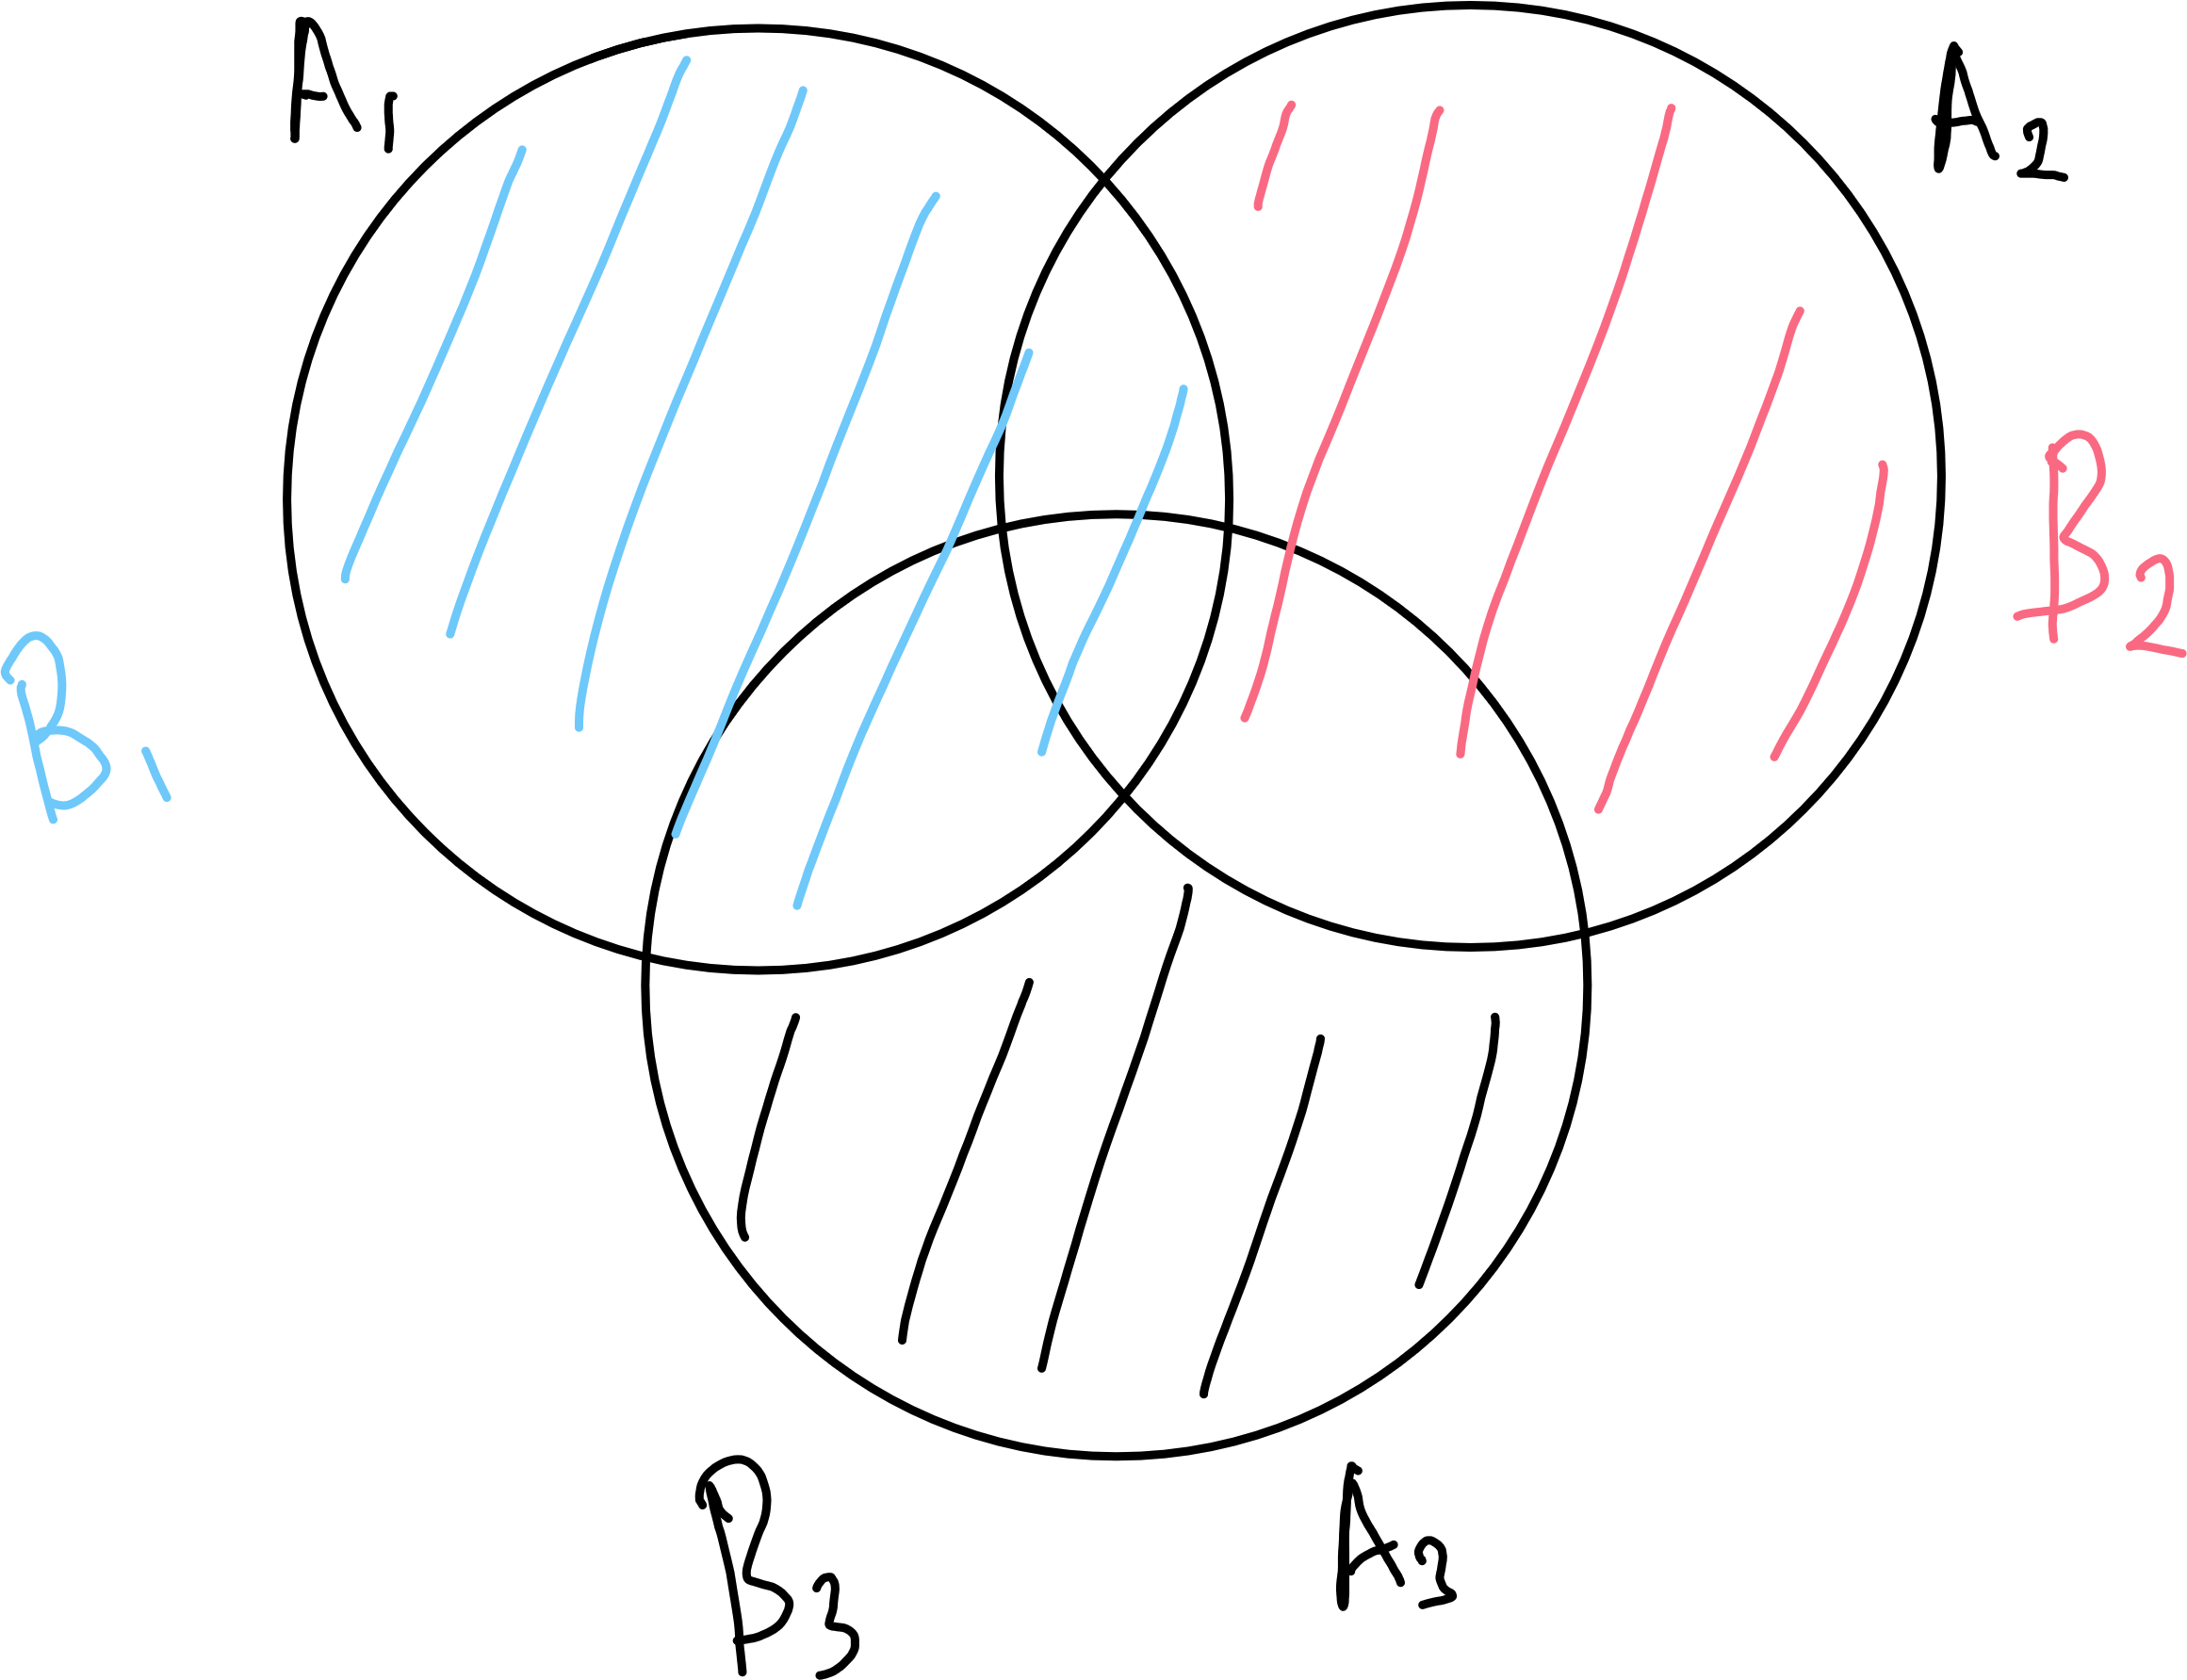
\includegraphics[height=5cm]{03-subadditivity} \par}
    So
    \begin{itemize}
        \item $\bigcup_{n \in \mathbb{N}} B_n = \bigcup_{n \in \mathbb{N}} A_n$.
        \item $(B_n)_{n \in \mathbb{N}}$ is disjoint (by construction).
        \item $B_n \subseteq A_n \implies \underbracket{\mathbb{P}(B_n) \leq \mathbb{P}(A_n)}_ {\text{Q4, Sheet 1}}$
    \end{itemize} 
    \begin{align*}
        \mathbb{P}\left(\bigcup_{n \in \mathbb{N}} A_n\right) = \mathbb{P}\left(\bigcup_{n \in \mathbb{N}} B_n\right) \underset{P3 \text{ on } (B_n)}{=} \sum_{n \in \mathbb{N}}  \mathbb{P}\left(B_n\right) \leq \sum_{n \in \mathbb{N}} \mathbb{P}\left(A_n\right)
    \end{align*} 
\end{proof} 

\subsection{Continuity}

\begin{proposition}[Continuity]
    Let $(A_n)_{n \in \mathbb{N}}$ be an increasing sequence of events in $\mathcal{F}$, i.e. $A_n \subseteq A_{n + 1} \quad \forall \; n$. 
    Then $\mathbb{P}(A_n) \leq \mathbb{P}(A_{n + 1})$.
    So $\mathbb{P}(A_n)$ converges as $n \to \infty$.\footnote{As probabilities are bounded above by 1 and increasing.}

    \emph{In fact:} $\lim_{n \to \infty} \mathbb{P}(A_n) = \mathbb{P} \left(\bigcup_{n \in \mathbb{N}} A_n \right)$.
\end{proposition} 

For motivation try Q6, Sheet 1.

\begin{figure}[h] 
    \centering 
    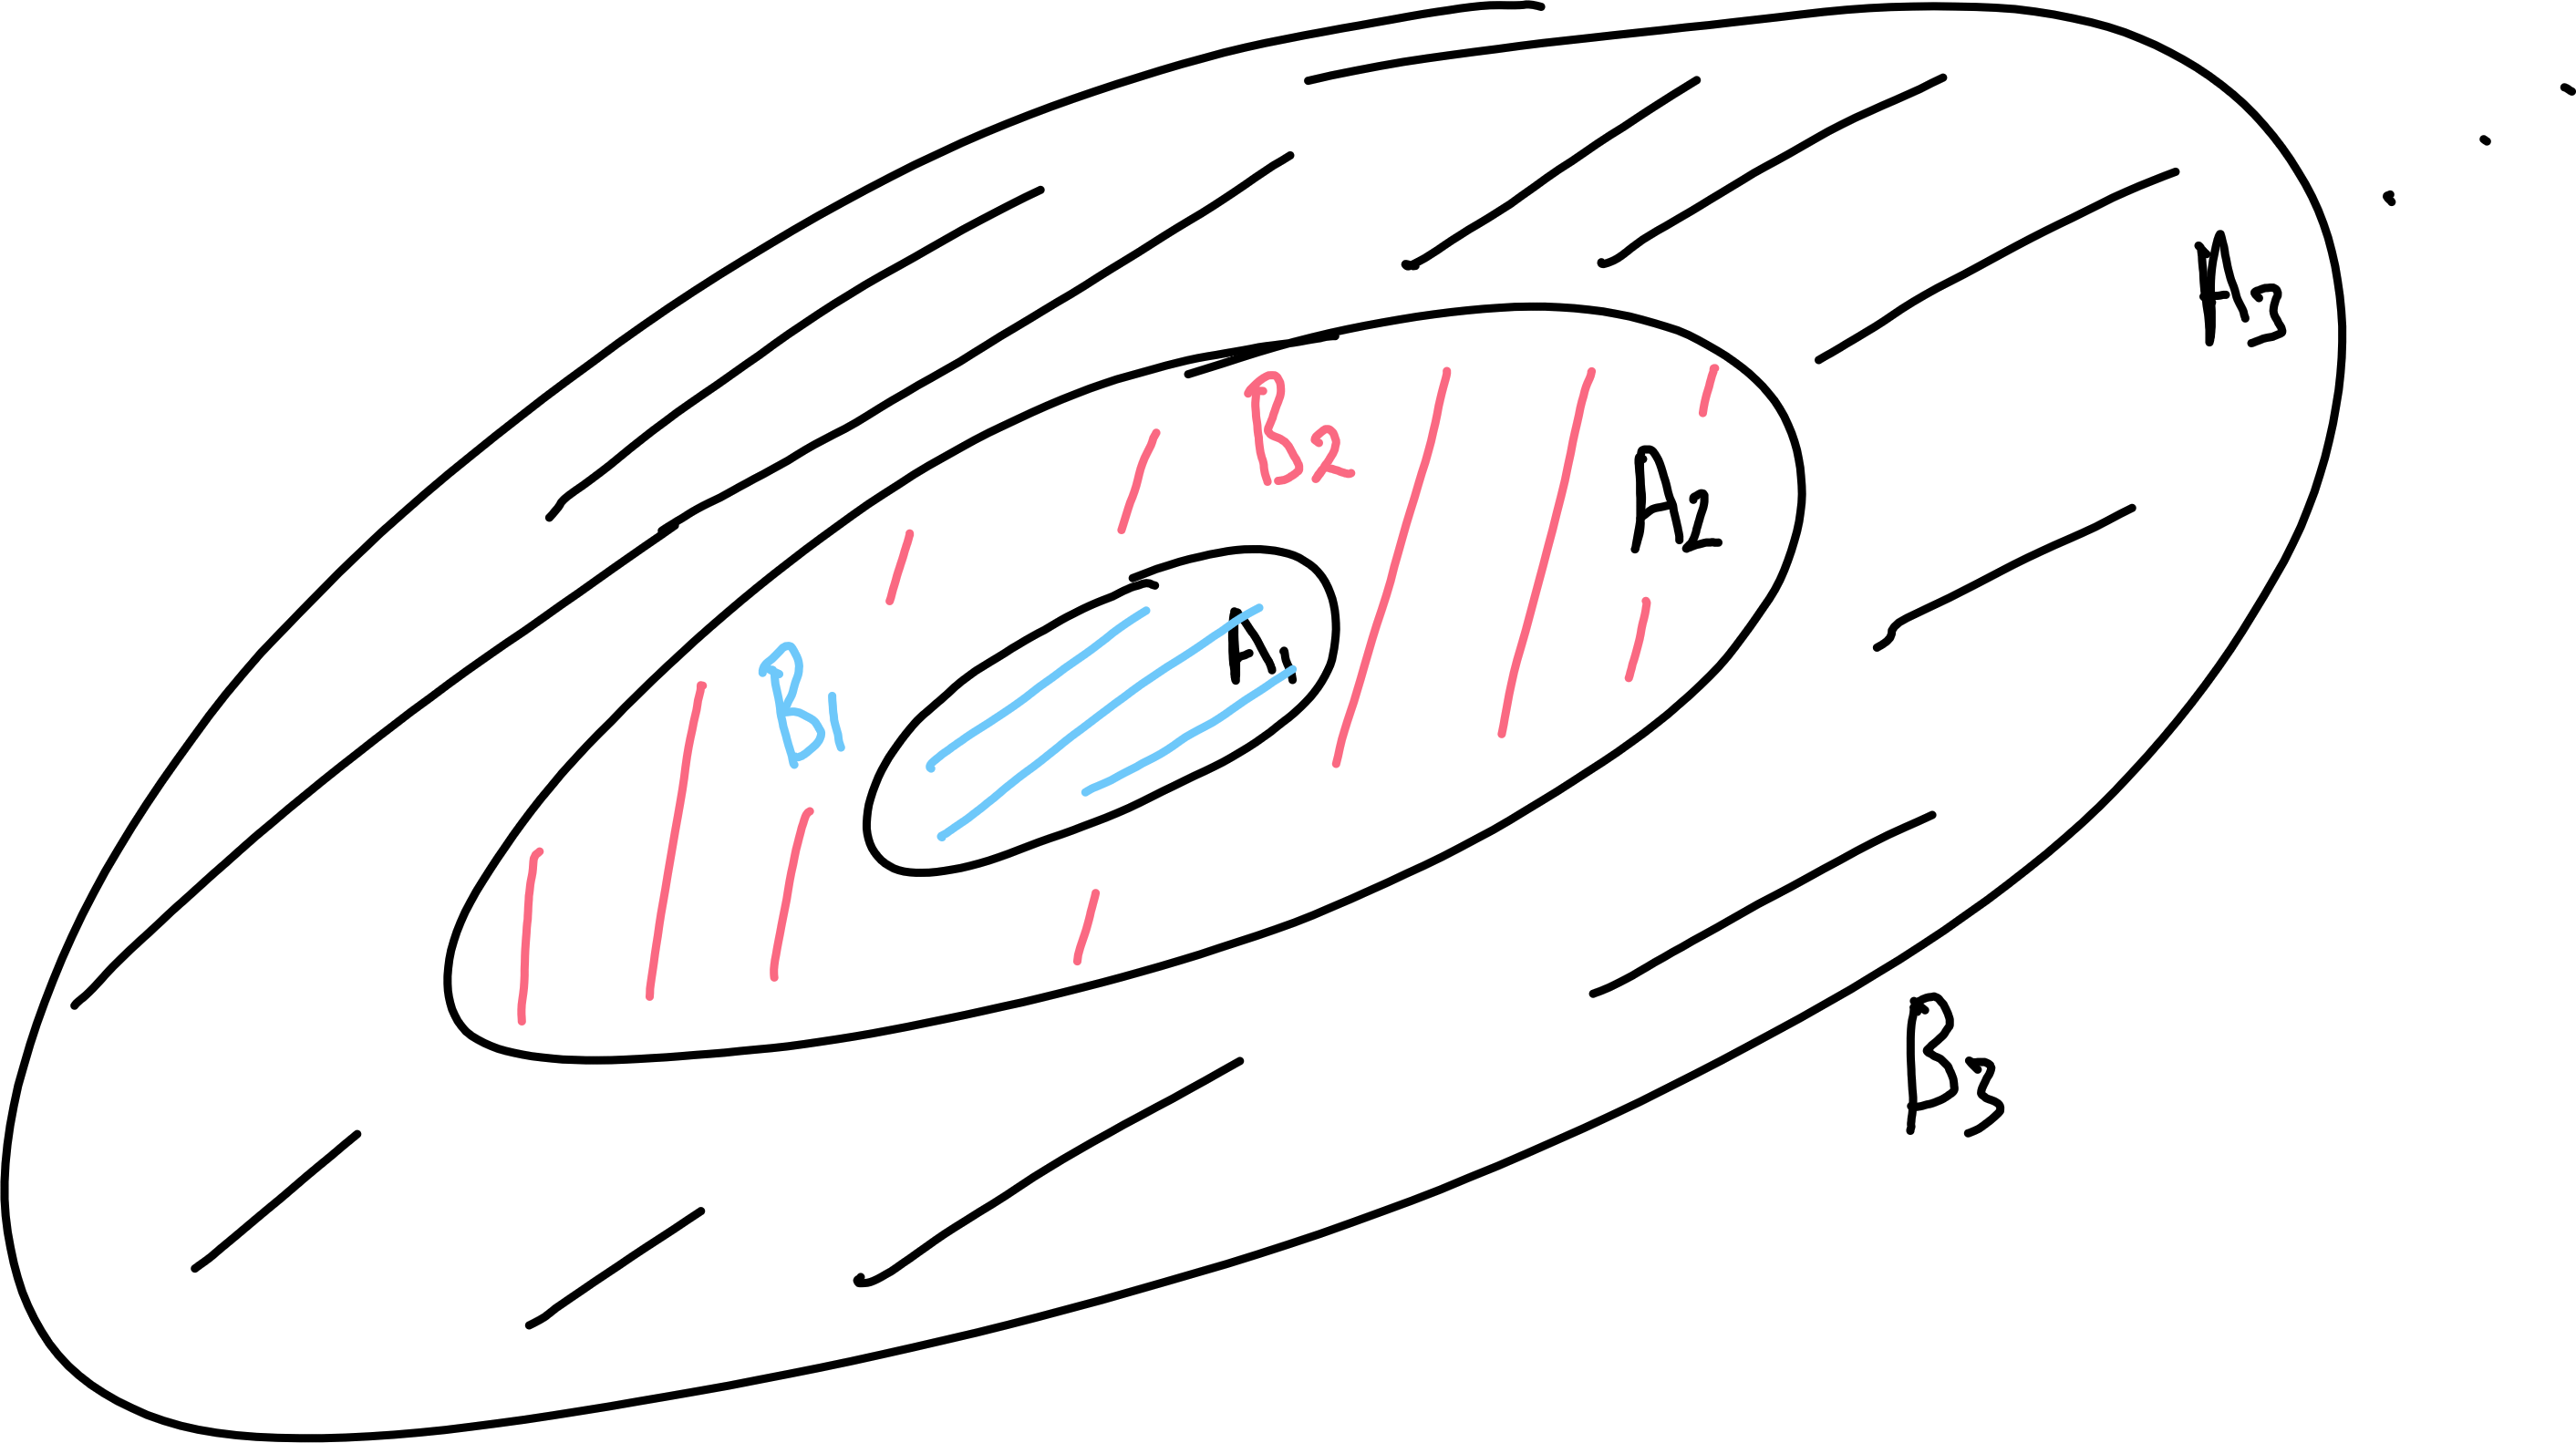
\includegraphics[height=5cm]{03-continuity} 
\end{figure}

\begin{proof}
    Let us reuse the $B_n$s from the previous subsection.
    \begin{itemize}
        \item $\bigcup_{k = 1}^n B_k = A_n$ (disjoint union).
        \item $\bigcup_{n \in \mathbb{N}} B_n = \bigcup_{n \in \mathbb{N}} A_n$
    \end{itemize} 
    \begin{align*}
        \mathbb{P}(A_n) &= \sum_{k=1}^{n} \mathbb{P}(B_k) \overset{n \to \infty}{\to} \sum_{k \geq 1} \mathbb{P}(B_k) = \mathbb{P} \left(\bigcup_{n \in \mathbb{N}} B_n \right) = \mathbb{P} \left(\bigcup_{n \in \mathbb{N}} A_n \right) 
    \end{align*} 
\end{proof} 

\subsection{Inclusion-Exclusion Principle}

Background: $\mathbb{P}(A \cup B) = \mathbb{P}(A) + \mathbb{P}(B) - \mathbb{P}(A \cap B)$. \\
Similarly: $A, B, C \in \mathcal{F}$
\begin{align*}
    \mathbb{P}(A \cup B \cup C) &= \mathbb{P}(A) + \mathbb{P}(B) + \mathbb{P}(C) - \mathbb{P}(A \cup B) - \mathbb{P}(B \cup C) - \mathbb{P}(C \cup A) + \mathbb{P}(A \cap B \cap C).
\end{align*} 

\begin{proposition}[Inclusion-Exclusion Principle] \label{prp:IEP}
    Let $A_1, \dots, A_n \in \mathcal{F}$, then:
    \begin{align*}
        \mathbb{P} \left(\bigcup_{i = 1}^n A_i \right) = &\sum_{i=1}^{n} \mathbb{P}(A_i) - \sum_{1 \leq i_1 < i_2 \leq n} \mathbb{P}(A_{i_1} \cap A_{i_2}) + \sum_{1 \leq i_1 < i_2 < i_3 \leq n} \mathbb{P}(A_{i_1} \cap A_{i_2} \cap A_{i_3}) - \dots \\ &+ (-1)^{n + 1} \mathbb{P}(A_1 \cap \dots \cap A_n) \\
        = &\sum_{\substack{I \subset \{1, \dots, n\} \\ I \neq \emptyset} } (-1)^{|I| + 1} \mathbb{P} \left( \bigcap_{i \in I} A_i \right)
    \end{align*}
    Note: $\sum_{1 \leq i_1 < i_2 \leq n}$ is the sum of all triples that are distinct and unordered.
\end{proposition}

\begin{proof}
    By induction. For $n=2$ it holds (Q4e, Sheet 1).
    \begin{align*}
        \mathbb{P}\left( \bigcup_{i = 1}^n A_i \right) &= \mathbb{P}\left(\left(\bigcup_{i = 1}^{n-1} A_i \right) \cup A_n \right) 
        \intertext{Using $n = 2$ case we get:}
        &= \mathcolor{blue}{\mathbb{P}\left( \bigcup_{i = 1}^{n - 1} A_i \right)} + \mathbb{P}(A_n) - \mathcolor{violet}{\mathbb{P}\left(\left(\bigcup_{i = 1}^{n-1} A_i \right) \cap A_n \right)} \\
        \intertext{We want to break down the final element on the RHS}
        \text{Idea: } \left(\bigcup_{i = 1}^{n-1} A_i \right) \cap A_n &= \bigcup_{i = 1}^{n - 1} \left(\mathcolor{red}{A_i \cap A_n} \right) \\
        \intertext{If we apply IEP to $\bigcup_{i = 1}^{n - 1} \left(\mathcolor{red}{A_i \cap A_n} \right)$ we need to calculate $\bigcap_{i \in J} \left(\mathcolor{red}{A_i \cap A_n} \right)$}
        \bigcap_{i \in J} \left(\mathcolor{red}{A_i \cap A_n} \right) &= \mathcolor{violet}{\bigcap_{i \in J \cup \{n\}} A_i}, \hspace{2cm} J \subset \{1, \dots, n - 1\} \\
        \\
        \mathbb{P}\left(\bigcup_{i = 1}^n A_i \right) &= \underbracket{\mathcolor{blue}{\sum_{\substack{J \subset \{1, \dots, n - 1\} \\ J \neq \emptyset}} (-1)^{|J| + 1} \mathbb{P} \left( \bigcap_{i \in J} A_i \right)}}_{n - 1 \text{ case}} + \mathbb{P}(A_n) \\
        &- \underbracket{\mathcolor{violet}{\sum_{\substack{J \subset \{1, \dots, n - 1\} \\ J \neq \emptyset}} (-1)^{|J| + 1} \mathbb{P} \left( \bigcap_{i \in J \cup \{n\}} A_i \right)}}_{n - 1 \text{ case on } (A_i \cap A_n)} \\
        J \cup \{n\} &\mapsto I. \\
        -(-1)^{|J| + 1} &\mapsto (-1)^{|I| + 1} \\
        &= \underbracket{\mathcolor{blue}{\sum_{\substack{I \subset \{1, \dots, n - 1\} \\ I \neq \emptyset}} (-1)^{|I| + 1} \mathbb{P} \left( \bigcap_{i \in I} A_i \right)}}_{\text{Just changed the labels}} + \mathbb{P}(A_n) \\
        &+ \mathcolor{violet}{\sum_{\substack{I \subset \{1, \dots, n\} \\ n \in I,\ |I| > 2}} (-1)^{|I| + 1} \mathbb{P} \left( \bigcap_{i \in I} A_i \right)} \\
        &= \sum_{\substack{I \subset \{1, \dots, n\} \\ I \neq \emptyset}} (-1)^{|I| + 1} \mathbb{P} \left( \bigcap_{i \in I} A_i \right).
    \end{align*}
    Let us check that we have indeed counted all subsets $I$.
    \begin{itemize}
        \item $\displaystyle \mathcolor{blue}{\sum_{\substack{I \subset \{1, \dots, n - 1\} \\ I \neq \emptyset}} (-1)^{|I| + 1} \mathbb{P} \left( \bigcap_{i \in I} A_i \right)}$ accounts for all subsets where $n \notin I$.
        \item $\mathbb{P}(A_n)$ accounts for $\{n\}$
        \item $\displaystyle \mathcolor{violet}{\sum_{\substack{I \subset \{1, \dots, n\} \\ n \in I,\ |I| > 2}} (-1)^{|I| + 1} \mathbb{P} \left( \bigcap_{i \in I} A_i \right)}$ accounts for all subsets where $n \in I$ and $I \neq \{n\}$.
    \end{itemize} 
\end{proof}

\subsection{Bonferroni Inequalities}
\begin{question}
    What if you \emph{truncate} IEP (Inclusion-Exclusion Principle)?
\end{question} 

\begin{proposition}[Bonferroni Inequality]
    Recall: \nameref{prp:subadditivity} - $\mathbb{P}(\cup A_i) \leq \sum \mathbb{P}(A_i)$.
    \begin{align*}
        \mathbb{P}\left(\bigcup_{i=1}^n A_i\right) &\leq \sum_{k = 1}^{\mathcolor{red} r} (-1)^{k+1} \sum_{i_1<i_2<\dots<i_k} \mathbb{P}(A_{i_1} \cap \dots \cap A_{i_k}) \quad \text{ if } \mathcolor{red} r \text{ is odd} \\
        \mathbb{P}\left(\bigcup_{i=1}^n A_i\right) &\geq \sum_{k = 1}^{\mathcolor{red} r} (-1)^{k+1} \sum_{i_1<i_2<\dots<i_k} \mathbb{P}(A_{i_1} \cap \dots \cap A_{i_k}) \quad \text{ if } \mathcolor{red} r \text{ is even}
    \end{align*} 
\end{proposition} 

\begin{proof}
    By induction on $r$ and $n$. Let $r$ be odd
    \begin{align*}
        \mathbb{P}\left( \bigcup_{i = 1}^n A_i \right) &= \mathcolor{blue}{\mathbb{P}\left( \bigcup_{i = 1}^{n - 1} A_i \right)} + \mathbb{P}(A_n) - \mathcolor{violet}{\mathbb{P} \left( \bigcup_{i = 1}^{n - 1} \left(A_i \cap A_n \right) \right)} \\
        \mathcolor{blue}{\mathbb{P}\left( \bigcup_{i = 1}^{n - 1} A_i \right)} &\leq \underbracket{\mathcolor{blue}{\sum_{\substack{J \subset \{1, \dots, n - 1\} \\ 1 \leq |J| \leq r}} (-1)^{|J| + 1} \mathbb{P} \left( \bigcap_{i \in J} A_i \right)}}_\text{$n - 1$ case.} \\
        \mathcolor{violet}{\mathbb{P} \left( \bigcup_{i = 1}^{n - 1} \left(A_i \cap A_n \right) \right)} &\geq \underbracket{\mathcolor{violet}{\sum_{\substack{J \subset \{1, \dots, n - 1\} \\ 1 \leq |J| \leq r - 1 \footnote{$J$ doesn't include $n$ and we only want $r$ elements in the intersection} }} (-1)^{|J| + 1} \mathbb{P} \left( \bigcap_{i \in J \cup \{n\}} A_i \right)}}_\text{$r  - 1$ case on $(A_i \cap A_n)$}
        \intertext{Using the same rearranging as in the proof of \nameref{prp:IEP}}
        \mathbb{P}\left( \bigcup_{i = 1}^n A_i \right) &\leq \sum_{\substack{I \subset \{1, \dots, n\} \\ 1 \leq |I| \leq r}} (-1)^{|I| + 1} \mathbb{P} \left( \bigcap_{i \in I} A_i \right).
    \end{align*}
    The case of $r$ being even is similar, simply note all three inequalities are reversed.
\end{proof} 

\begin{question}
    When is it good to truncate at e.g. r = 2?
\end{question}

\subsection{Counting with IEP}

Uniform probability measure on $\Omega$, $|\Omega| < \infty$.
$\mathbb{P}(A) = \frac{|A|}{|\Omega|} \quad \forall \; A \subseteq \Omega$.
Then $\forall \; A_1, \dots, A_n \subseteq \Omega$
\begin{align*}
    |A_1 \cup \dots \cup A_n| = \sum_{k=1}^{n} (-1)^{k + 1} \sum_{i_1 < \dots < i_k} |A_i \cap \dots \cap A_{i_k}| 
\end{align*} (and similarly for Bonferroni Inequalities).

\begin{example}[Surjections]
    What is the probability that a function $f: \{1,\dots, n\} \to \{1,\dots,m\},\ n \geq m$ is a surjection?
    Let $\Omega = \{f: \{1,\dots,n\} \to \{1,\dots,m\}\}$ and $A = \{f \in \Omega: \operatorname{Image}(f) = \{1, \dots, m\}\}$.\\
    $\forall \; i \in \{1,\dots,m\}$ define $B_i = \{f \in \Omega: i\not \in \operatorname{Image}(f)\}$.

    \emph{Key observations}:
    \begin{itemize}
        \item \begin{align*}
            A &= B_1^c \cap \dots B_m^c \\
            &= (B_1 \cup \dots \cup B_m)^c
        \end{align*} 
        \item $|B_{i_1} \cap \dots \cap B_{i_k}|$ is nice to calculate.
        \begin{align*}
            |B_{i_1} \cap \dots \cap B_{i_k}| &= | \{ f \in \Omega : i_1, \dots, i_k \notin \operatorname{Image}(f) | \\
            &= (m - k)^n \\
            IEP \to |B_1 \cup \dots \cup B_m| &= \sum_{k=1}^{m} (-1)^{k + 1} \sum_{i_1 < \dots < i_k} \underbracket{|B_{i_1} \cap \dots \cap B_{i_k}|}_\text{same for all $i_1, \dots, i_k$}\\
            &= \sum_{k=1}^{m} (-1)^{k+1} \binom{m}{k} (m - k)^n \\
            |A| &= m^n - |B_{i_1} \cap \dots \cap B_{i_k}| \\
            &= \sum_{k=0}^m (-1)^k \binom{m}{k} (m - k)^n 
        \end{align*} 
    \end{itemize}
\end{example} 

\begin{example}[Derangements]
    What is the probability that a permutation has no fixed points? Derangements can be useful in a Secret Santa. \\
    $\Omega = \left\{\text{permuations of } \{1, \dots, n\} \right\}$ and the derangements, $D$, are $\{\sigma \in \Omega : \sigma(i) \neq i \quad \forall \; i = 1, \dots, n\}$.
    %
    \begin{question}
        Is $\mathbb{P}(D) = \frac{|D|}{|\Omega|}$ large or small (e.g. when $n \to \infty$?)
    \end{question} 
    %
    $\forall \; i \in \{1, \dots, n\} : A_i = \{\sigma \in \Omega : \sigma(i) = i\}$. \\
    \emph{Key observations}:
    \begin{itemize}
        \item $D = A_1^c \cap \dots A_n^c = \left(\bigcup_{i = 1}^n A_i \right)^c.$
        \item \begin{align*}
            \mathbb{P}(A_{i_1} \cap \dots \cap A_{i_k}) &= \frac{(n - k)!}{n!} \\
            IEP \to \mathbb{P}\left(\bigcup_{i = 1}^n A_i \right) &= \sum_{k=1}^{n} (-1)^{k + 1} \sum_{i_1 < \dots < i_k} \mathbb{P}(A_{i_1} \cap \dots \cap A_{i_k}) \\
            &= \sum_{k=1}^{n} (-1)^{k+1} \binom{n}{k} \frac{(n - k)!}{n!} \\
            &= \sum_{k=1}^{n} (-1)^{k+1} \frac{1}{k!} \\
            \mathbb{P}(D) &= 1 - \mathbb{P}\left(\bigcup_{i = 1}^n A_i \right) \\
            &= 1 - \sum_{k=1}^{n} \frac{(-1)^{k+1}}{k!} \\
            &= \sum_{k=0}^{n} \frac{(-1)^{k}}{k!} \\
            \lim_{n \to \infty} \mathbb{P}(D) &= \sum_{k=0}^{\infty} \frac{(-1)^{k+1}}{k!} \\
            &= e^{-1} \approx 0.37.
        \end{align*} 
    \end{itemize}

    \begin{remark} \mbox{}
        \begin{itemize}
            \item What if instead $\Omega' = \{\text{all functions } f : \{1, \dots, n\} \text{ to itself} \}$?
            \begin{align*}
                D &= \{f \in \Omega' : f(i) \neq i \quad \forall \; i = 1, \dots, n\}. \\
                \mathbb{P}(D) &= \frac{(n-1)^n}{n^n} \\
                &= \left(1 - \frac{1}{n}^n \right) \\
                \lim_{n \to \infty} D &= e^{-1}.
            \end{align*} 
            \item We would liked to have calculated $\mathbb{P}(D)$ by doing $\left(\frac{n - 1}{n}\right)^n$ as we have $n$ choices each with probability $\frac{n - 1}{n}$.
            We will be allowed to do this soon! See \Cref{exm:conditional} 
            \item $f(i)$ is a random quantity associated to $\Omega$.
            We will be allowed to study $f(i)$ as a \emph{random variable} soon.
            \item We are allowed to toss a fair coin $n$ times, $\Omega = \{H, T\}^n$.
            But we have not yet studied tossing an unfair coin $n$ times.
        \end{itemize} 
    \end{remark} 
\end{example} 

\subsection{Independence}
$(\Omega, \mathcal{F}, \mathbb{P})$ as before.

\begin{definition}[Indepence]
    Events $A, B \in \mathcal{F}$ are \vocab{independent} ($A \indep B$) if
    \begin{align*}
        \mathbb{P}(A \cap B) &= \mathbb{P}(A) \mathbb{P}(B).
    \end{align*} 
    A countable\footnote{including finite} collection of events $(A_n)$ are \vocab{independent} if $\forall$ distinct $i_1, \dots, i_k$\footnote{$k$ is finite} we have:
    \begin{align*}
        \mathbb{P}(A_{i_1} \cap \dots \cap A_{i_k}) &= \prod_{j = 1}^k \mathbb{P}(A_{i_j}).
    \end{align*} 
\end{definition} 

\begin{remark}[Caution]
    ``Pairwise independence'' does not imply independence.
\end{remark} 

\begin{example} ~\vspace*{-1.5\baselineskip}
    \begin{align*}
        \Omega &= \{(H, H), (H, T), (T, H), (T, T)\} \\
        \mathbb{P}(\{\omega\}) &= \frac{1}{4} \quad \forall \; \omega \in \Omega. \\
        A &= \text{first coin is $H$} = \{(H, H), (H, T)\}. \\
        B &= \text{second coin is $H$} = \{(T, H), (H, H)\}. \\
        C &= \text{both coins have the same outcome} = \{(T, T), (H, H)\}. \\
        \mathbb{P}(A) &= \mathbb{P}(B) = P(C) = \frac{1}{2}. \\
        A \cap B &= A \cap C = B \cap C = \{(H, H)\}. \\
        \mathbb{P}(A \cap B) &= \mathbb{P}(A \cap C) = \mathbb{P}(B \cap C) = \frac{1}{4}. \quad \text{Pairwise independence } \checkmark \\
        \mathbb{P}(A \cap B \cap C) &= \frac{1}{4} \neq \mathbb{P}(A) \mathbb{P}(B) \mathbb{P}(C). \quad \text{Independence } \times
    \end{align*} 
\end{example} 

\begin{example}[Independence] ~\vspace*{-1.5\baselineskip}
    \begin{itemize}
        \item \begin{align*}
            \Omega' &= \{\text{all functions } f : \{1, \dots, n\} \text{ to itself} \\
            A_i &= \{f \in \Omega' : f(i) = i\}. \\
            \mathbb{P}(A_i) &= \frac{n^{n -1}}{n^n} = \frac{1}{n} \\
            \mathbb{P}(A_{i_1} \cap \dots \cap A_{i_k}) &= \frac{n^{n -k}}{n^n} \\
            &= \frac{1}{n^k} \\
            &= \prod_{j = 1}^k \mathbb{P}(A_{i_j})
        \end{align*} 
        Here: $(A_i)$ are independent events.
        \item \begin{align*}
            \Omega &= \left\{\sigma : \text{ permutation of } \{1, \dots, n\} \right\} \\
            A_i &= \{ \sigma \in \Omega : \sigma(i) = i \} \\
            \mathbb{P}(A_i) &= \frac{(n - 1)!}{n!} = \frac{1}{n}. \\
            i \neq j \quad \mathbb{P}(A_i \cap A_j) &= \frac{(n - 2)!}{n!} \\
            &= \frac{1}{n(n - 1)} \\
            &\neq \mathbb{P}(A_i) \mathbb{P}(A_j)
        \end{align*} 
        Here: $(A_i)$ are not independent events.
    \end{itemize} 
\end{example} 

\subsubsection{Properties}
\begin{claim}
    If $A$ is independent of $B$, then $A$ is also independent of $B^c$.
\end{claim} 

\begin{proof}
    \begin{align*}
        \mathbb{P}(A \cap B^c) &= \mathbb{P}(A) - \mathbb{P}(A \cap B) \\
        &= \mathbb{P}(A) - \mathbb{P}(A)\mathbb{P}(B) \\
        &= \mathbb{P}(A) [1 - \mathbb{P}(B)] \\
        &= \mathbb{P}(A) \mathbb{P}(B^C)
    \end{align*}  
\end{proof} 

\begin{claim}
    $A$ is independent of $B = \Omega$ and of $C = \emptyset$
\end{claim} 

\begin{proof}
    $\mathbb{P}(A \cap \Omega) = P(A) = \mathbb{P}(A) \underbracket{\mathbb{P}(\Omega)}_{= 1}$ and so $A \indep \emptyset$ by Claim 1.
\end{proof} 

\subsection{Conditional Probability}
$(\Omega, \mathcal{F}, \mathbb{P})$ as before.

Consider $B \in \mathcal{F}$ with $\mathbb{P}(B) > 0,\ A \in \mathcal{F}$

\begin{definition}[Conditional Probability]
    The \vocab{conditional probability} of $A$ given $B$ is $\mathbb{P}(A \mid B) = \frac{\mathbb{P}(A \cap B)}{\mathbb{P}(B)}$
\end{definition} 
\color{blue} ``The probability of $A$ is we know $B$ happened". (e.g. revealing information in succession)

\begin{example}
    $A, B$ independent.
    \begin{align*}
        \mathbb{P}(A \mid B) = \frac{\mathbb{P}(A \cap B)}{\mathbb{P}(B)} = \frac{\mathbb{P}(A) \mathbb{P}(B)}{\mathbb{P}(B)} = \mathbb{P}(A)
    \end{align*} 
    \color{blue}``Knowing whether $B$ happened doesn't affect the probability of $A$".
\end{example} 
\color{black}

\subsubsection{Properties}

\begin{itemize}
    \item P1 - $\mathbb{P}(A \mid B) \geq 0$ 
    \item P2 - $\mathbb{P}(B \mid B) = 1 = \mathbb{P}(\Omega \mid B)$
    \item P3 - $(A_n)$ disjoint events $\in \mathcal{F}$:
    \begin{claim} ~\vspace*{-1.5\baselineskip}
        \begin{align*}
            \mathbb{P}\left(\bigcup_{n \in \mathbb{N}} A_n \mid B\right) = \sum_{n \in \mathbb{N}} \mathbb{P}(A_n \mid B)
        \end{align*} 
    \end{claim} 

    \begin{proof}
        \begin{align*}
            \mathbb{P}\left(\bigcup_{n \in \mathbb{N}} A_n \mid B\right) &= \frac{\mathbb{P}\left( \left( \bigcup_n A_n \right) \cap B \right)}{\mathbb{P}(B)} \\
            &= \frac{\mathbb{P}\left( \bigcup_n \left(A_n \cap B \right) \right)}{\mathbb{P}(B)}, \quad \mathcolor{blue}{\cup (A_n \cap B) \text{ is a disjoint union}} \\
            &= \frac{\sum_n \mathbb{P}(A_n \cap B)}{\mathbb{P}(B)} \\
            &= \sum_{n \in \mathbb{N}} \mathbb{P}(A_n \mid B)
        \end{align*} 

        Summary: Use definition and apply P1, P2, P3 to the numerator.
    \end{proof} 
\end{itemize} 

$\mathbb{P}(\bullet \mid B)$ is a function from $\mathcal{F} \to [0, 1]$ that satisfies the rules to be a probability measure on $\Omega$.

\begin{aside}{Aside?}
    Consider $\Omega' = B$ (especially in finite or countable setting).
    Let $\mathcal{F}' = \mathcal{P}(B)$.
    Then $\left(\Omega', \mathcal{F}', \mathbb{P}(\bullet \mid B)\right)$ also satisfies rules to be a probability measure on $\Omega'$.
\end{aside} 

\begin{align}
    \mathbb{P}(A \cap B) &= \mathbb{P}(A) \mathbb{P}(B \mid A) \label{eq:union} \\
    \mathbb{P}(A_1 \cap A_2 \cap \dots \cap A_n) &= \mathbb{P}(A_1) \mathbb{P}(A_2 \mid A_1) \mathbb{P}(A_3 \mid A_1 \cap A_2) \dots \mathbb{P}(A_n \mid A_1 \cap \dots \cap A_{n - 1}) \notag
\end{align} 

\begin{example} \label{exm:conditional}
    Uniform choice of a permutation $(\sigma(1), \sigma(2), \dots, \sigma(n)) \in \Sigma_n$.
    \begin{claim} ~\vspace*{-1.5\baselineskip} \label{clm:perms}
        \begin{align*}
            \mathbb{P}\left(\sigma(k) = i_k \mid \sigma(1) = i, \dots, \sigma(k - 1) = i_{k-1} \right), \quad i_1, \dots, i_{k-1} \text{ distinct.} \\
            = \begin{cases}
                0 & \text{if } i_k \in \{i_1, \dots, i_{k-1} \}. \\
                \frac{1}{n - k + 1}\footnote{This is an example of \nameref{Ordered compositions}} & \text{else}
            \end{cases} 
        \end{align*} 
    \end{claim} 

    \begin{proof}
        \begin{align*}
            \mathbb{P}\left(\sigma(k) = i_k \mid \sigma(1) = i, \dots, \sigma(k - 1) = i_{k-1} \right) &= \frac{\mathbb{P}(\sigma(1) = i, \dots, \sigma(k) = i_k)}{\mathbb{P}(\sigma(1) = i, \dots, \sigma(k - 1) = i_{k-1})} \\
            &= \frac{\frac{(n - k)!}{n!}}{\frac{(n - k + 1)!}{n!}} \\
            &= \frac{(n - k)!}{(n - k + 1)!} \\
            &= \frac{1}{n - k + 1} \\
            \mathbb{P}(\sigma(1) = i, \dots, \sigma(k) = i_k) &= 0 \quad \text{if } i_k \in \{i_1, \dots, i_{k-1} \}.
        \end{align*} 
    \end{proof} 
\end{example} 

\subsubsection{Law of Total Probability and Bayes' Formula}

\begin{definition}[Partition]
    $(B_1, B_2, \dots)\footnote{finite or countable} \in \Omega$ is a \vocab{partition} of $\Omega$ if:
    \begin{itemize}
        \item $\Omega = \bigcup_n B_n$
        \item $(B_n)$ are disjoint
    \end{itemize} 
\end{definition} 

\begin{theorem}[Law of Total Probability] \label{thm:ltp}
    $(B_n)$ a finite or countable partition of $\Omega$ with $B_n \in \mathcal{F} \ \forall \; n$ s.t. $\mathbb{P}(B_n) > 0$.
    Then $\forall \; A \in \mathcal{F}$:
    \begin{align*}
        \mathbb{P}(A) &= \sum_n \mathbb{P}(A \mid B_n) \mathbb{P}(B_n).
    \end{align*}  
    Also know as ``Partition Theorem".
\end{theorem} 

\begin{proof}
    Note that $\bigcup_n \left(A \cap B_n \right) = A$.
    \begin{align*}
        \mathbb{P}(A) &= \sum_{n \in \mathbb{N}} \mathbb{P}(A \cap B_n) \\
        &= \sum_n \mathbb{P}(A \mid B_n) \mathbb{P}(B_n) \quad \text{by \Cref{eq:union}}
    \end{align*} 
\end{proof} 

\begin{theorem}[Bayes' Formula] \label{thm:bayes}
    Same setup as above
    \begin{align*}
        \mathbb{P}(B_n \mid A) &= \frac{\mathbb{P}(A \cap B_n)}{\mathbb{P}(A)} \\
        &= \frac{\mathbb{P}(A \mid B_n) \mathbb{P}(B_n)}{\sum_m \mathbb{P}(A \mid B_m) \mathbb{P}(B_m)}.
    \end{align*} 
    Let $n = 2$: $\mathbb{P}(B \mid A) \mathbb{P}(A) = \mathbb{P}(A \mid B) \mathbb{P}(B) = \mathcolor{red}{\mathbb{P}(A \cap B)}$
\end{theorem} 

\begin{example}[Lecture course]
    Consider a Lecture course which has $2 / 3$ of the lectures on weekdays and $1 / 3$ on weekends.
    Let 
    \begin{align*}
        \mathbb{P}(\text{forget notes} \mid \text{weekday}) &= \frac{1}{8} \\
        \mathbb{P}(\text{forget notes} \mid \text{weekend}) &= \frac{1}{2}
    \end{align*} 
    What is $\mathbb{P}(\text{weekend} \mid \text{forget notes})$?
    Let $B_1 = \{\text{weekday}\}, B_2 = \{ \text{weekend} \}$ and $A = \{\text{forget notes}\}$. \\
    By LTP (\nameref{thm:ltp}): $\mathbb{P}(A) = \frac{2}{3} \times \frac{1}{8} + \frac{1}{3} \times \frac{1}{2} = \frac{1}{4}$. \\
    By \nameref{thm:bayes}: $\mathbb{P}(B_2 \mid A) = \frac{1}{3} \times \frac{1}{2} / \frac{1}{4} = \frac{2}{3}$.
\end{example}

\begin{example}[Disease Testing]
    Suppose $p$ are infected and $(1 - p)$ are not.
    $\mathbb{P}(\text{tests positive} \mid \text{infected}) = 1 - \alpha$ and $\mathbb{P}(\text{tests positive} \mid \text{not infected}) = \beta$ where $\alpha, \beta \in (0, 1)$.

    We want to work out $\mathbb{P}(\text{infected} \mid \text{test positive})$.

    By LTP: $\mathbb{P}(\text{test positive}) = p (1 - \alpha) + (1 - p) \beta$. \\
    By \nameref{thm:bayes}: $\mathbb{P}(\text{infected} \mid \text{test positive}) = \frac{p (1 - \alpha)}{p (1 - \alpha) + (1 - p) \beta}$.

    Suppose $p \ll \beta$ then $p(1 - \alpha) \ll (1 - p) \beta$ so $\mathbb{P}(\text{infected} \mid \text{test positive}) \sim \frac{p(1 - \alpha)}{(1 - p) \beta} \sim \frac{p}{\beta}$ which is small.
\end{example} 

\begin{example}[Simpson's Paradox]
    Scientists ask: do jelly beans make you tongue change colour?

    \begin{center}
        \begin{tabular}{ m{2cm} |c|c|c } 
         Oxford & Change & No change & \% change \\ 
         \hline
         Blue   & 15     &  22       & 41\% \\
         Green  & 5      &  8        & 38\%
        \end{tabular}
        $\Delta = 3\%$
    \end{center}
    \begin{center}
        \begin{tabular}{ m{2cm} |c|c|c } 
            Cambridge & Change & No change & \% change \\ 
            \hline
            Blue      & 10     &  3        & 77\% \\
            Green     & 23     &  14       & 62\%
        \end{tabular}
        $\Delta = 15\%$
    \end{center} 
    \begin{center}
        \begin{tabular}{ m{2cm} |c|c|c } 
        Total  & Change & No change & \% change \\ 
        \hline
        Blue   & 25     &  25       & 50\% \\
        Green  & 28     &  22       & 56\%
        \end{tabular}
        $\Delta = -6\%$
    \end{center}

    The conclusion from this example should be that the Cambridge methodology is different to the Oxford one rather than anything about blue/ green jelly beans.\footnote{Obviously this is a frivolous example however if we changed Oxford to November 2021, Cambridge to January 2021 and we were measuring vaccine efficacy for different vaccines we would get similar results. And it would be reasonable to conclude that the main underlying factor was a change in the viral landscape rather than waning efficacy.}

    Let $A = \{\text{change colour}\}$, $B = \{\text{blue}\}$, $B^C = \{\text{green}\}$, $C = \{\text{Cambridge}\}$, $C^c = \{\text{Oxford}\}$.
    \begin{align*}
        \mathbb{P}(A \mid B \cap C) &> \mathbb{P}(A \mid B^c \cap C) \\
        \mathbb{P}(A \mid B \cap C^c) &> \mathbb{P}(A \mid B^c \cap C^c) \\
        \centernot\implies \mathbb{P}(A \mid B) &> \mathbb{P}(A \mid B^c)
    \end{align*} 
\end{example} 

\begin{theorem}[Law of Total Probability for Conditional Probabilities]
    Suppose $C_1, C_2, \dots$ a partition of $B$.
    \begin{align*}
    \mathbb{P}(A \mid B) &= \sum_n \mathbb{P}(A \mid C_n) \mathbb{P}(C_n \mid B)
    \end{align*} 
\end{theorem} 

\begin{proof}
    \begin{align*}
        \mathbb{P}(A \mid B) &= \frac{\mathbb{P}(A \cap B)}{\mathbb{P}(B)} \\
        &= \frac{\mathbb{P}\left(A \cap \left( \bigcup_n C_n \right)\right)}{\mathbb{P}(B)} \\
        &= \frac{\mathbb{P}\left( \bigcup_n (A \cap C_n) \right)}{\mathbb{P}(B)} \\
        &= \frac{\sum_n \mathbb{P}(A \cap C_n)}{\mathbb{P}(B)} \\
        &= \frac{\sum_n \mathbb{P}(A \mid C_n) \mathbb{P}(C_n)}{\mathbb{P}(B)} \\
        &= \sum_n \mathbb{P}(A \mid C_n) \frac{\mathbb{P}(B \cap C_n)}{\mathbb{P}(B)} \quad C_n \subset B \implies B \cap C_n = C_n \\
        &= \sum_n \mathbb{P}(A \mid C_n) \mathbb{P}(C_n \mid B)
    \end{align*} 
\end{proof} 

\begin{aside}{Non Examinable}
    \emph{Special Case}: 
    \begin{itemize}
        \item If all $\mathbb{P}(C_n)$ are equal then so are $\mathbb{P}(C_n \mid B)$. Note $\sum_n \mathbb{P}(C_n \mid B) = 1$.
        \item If $\mathbb{P}(A \mid C_n)$ are all equal.
    \end{itemize} 

    Then $\mathbb{P}(A \mid B) = \mathbb{P}(A \mid C_n)$.

\end{aside} 

\begin{example}[Well-shuffled deck of cards]
    Uniformly chosen \emph{permutation}, $\sigma \in \Sigma_{52}$, of $52$ cards.
    $\{1, 2, 3, 4\}$ are \emph{aces}.
    Let $A = \{\sigma(1), \sigma(2) \text{ are aces}\}$, $B = \{\sigma(1) \text{ is an ace}\} = \{\sigma(1) \leq 4\}$, $C_1 = \{\sigma(1) = 1\} \dots C_4 = \{\sigma(1) = 4\}$.

    Note:
    \begin{itemize}
        \item \begin{align*}
            \mathbb{P}(A \mid C_i) &= \mathbb{P}(\sigma(2) \in \{1, 2, 3, 4\} \mid \sigma(1) = i) \quad i \leq 4 \\
            &= \frac{3}{51} \text{ by \Cref{clm:perms}}
        \end{align*} 
        \item $\mathbb{P}(C_1) = \dots = \mathbb{P}(C_4) = \frac{1}{52}$.
    \end{itemize} 
    So $\mathbb{P}(A \mid B) = \frac{3}{51}$ and $\mathbb{P}(A) = \mathbb{P}(B) \mathbb{P}(A \mid B) = \frac{4}{52} \times \frac{3}{51}$
\end{example}